Grandes volumenes de datos digitales son alamacenados día a día, en forma de noticias, blogs, páginas web, artículos científicos, libros, imágenes, sonido, video, redes sociales, etc. Volviéndose cada vez más difícil encontrar y descubrir lo que estamos buscando. Necesitamos herramientas computacionales que ayuden a organizar, buscar y entender grandes colecciones de datos.\\

Si pudieramos buscar y explorar documentos en base a sus temas, podríamos enfocar nuestra búsqueda en temas específicos o más amplios, podríamos observar como estos temas cambian en el tiempo o como se relacionan unos a otros. En vez de buscar documentos únicamente a través de palabras claves, podríamos primero hallar temas que son de nuestro interés, y luego examinar los documentos relacionados a ese tema. Por ejemplo, podríamos descubrir nuevas tendencias de investigación, analizar la evolución de la contigencia social, estudiar la efectividad de campañas publicitarias en base a la opinión de los consumidores, organizar y recomendar contenido en un blog, etc.\\

El objetivo del trabajo de tesis es desarrollar una metodología que permita descubrir tópicos en el tiempo, siendo capaz de modelar cambios tales como: nacimiento, muerte, evolución, división y fusión. Adicionalmente, que sea robusta a cambios en el vocabulario en el tiempo, permitiendo comparar tópicos entre épocas adyacentes a pesar que no posean un vocabulario común.

\section{Metodología Propuesta}
Los modelos de tópicos probabilísticos nos ayudan a descubrir los temas latentes (\textit{clusters}) en una colección de documentos, como estos temas están conectados unos a otros y cómo cambian en el tiempo. Permiten resumir un gran colección de documentos a través de sus temas y organizarlos entorno a estos.\\

Los modelos probabilísticos tratan un tópico como una distribución de probabilidad discreta sobre el vocabulario del corpus, siendo un práctica habitual interpretar un tópico a partir de sus $N$ palabras más probables. Por ejemplo, para $N=5$ las palabras más probables de un tópico son: \quotes{llaves}, \quotes{domicilio}, \quotes{individuos}, \quotes{casa} y \quotes{porton}, por lo que una etiqueta valida para este tópico podría ser \quotes{portonazo}.\\ 

En esta tesis se propone una metodología para el descubrimiento de tópicos en el tiempo. Esta metodología consiste en la discretización del corpus en épocas, el descubrimiento de tópicos en cada época mediante Hierarchical Dirichlet Process (HDP), la construcción de un grafo de similitud entre tópicos de épocas adyacentes, el cual permite modelar cambios entre los tópicos como: nacimiento, muerte, evolución, división y fusión. En contraste a trabajos anteriores, la metodología propuesta utiliza Word Mover's Distance (WMD) como medida de similitud entre tópicos. Esta medida destaca por su robustez ante tópicos que no poseen un vocabulario común, debido a que trabaja sobre el espacio de los \textit{word embeddings}.\\

\section{Caso de estudio}

Se escoge el problema del robo de vehículos o accesorios de vehículos como caso de estudio, debido a que es un problema que afecta a toda la sociedad en Chile y en el mundo, problema que se ha vuelto más relevante el último tiempo debido al crecimiento en el robo de vehículo motorizado y accesorios (ver Figura \ref{fig:antecedente}).\\ 

\begin{figure}
    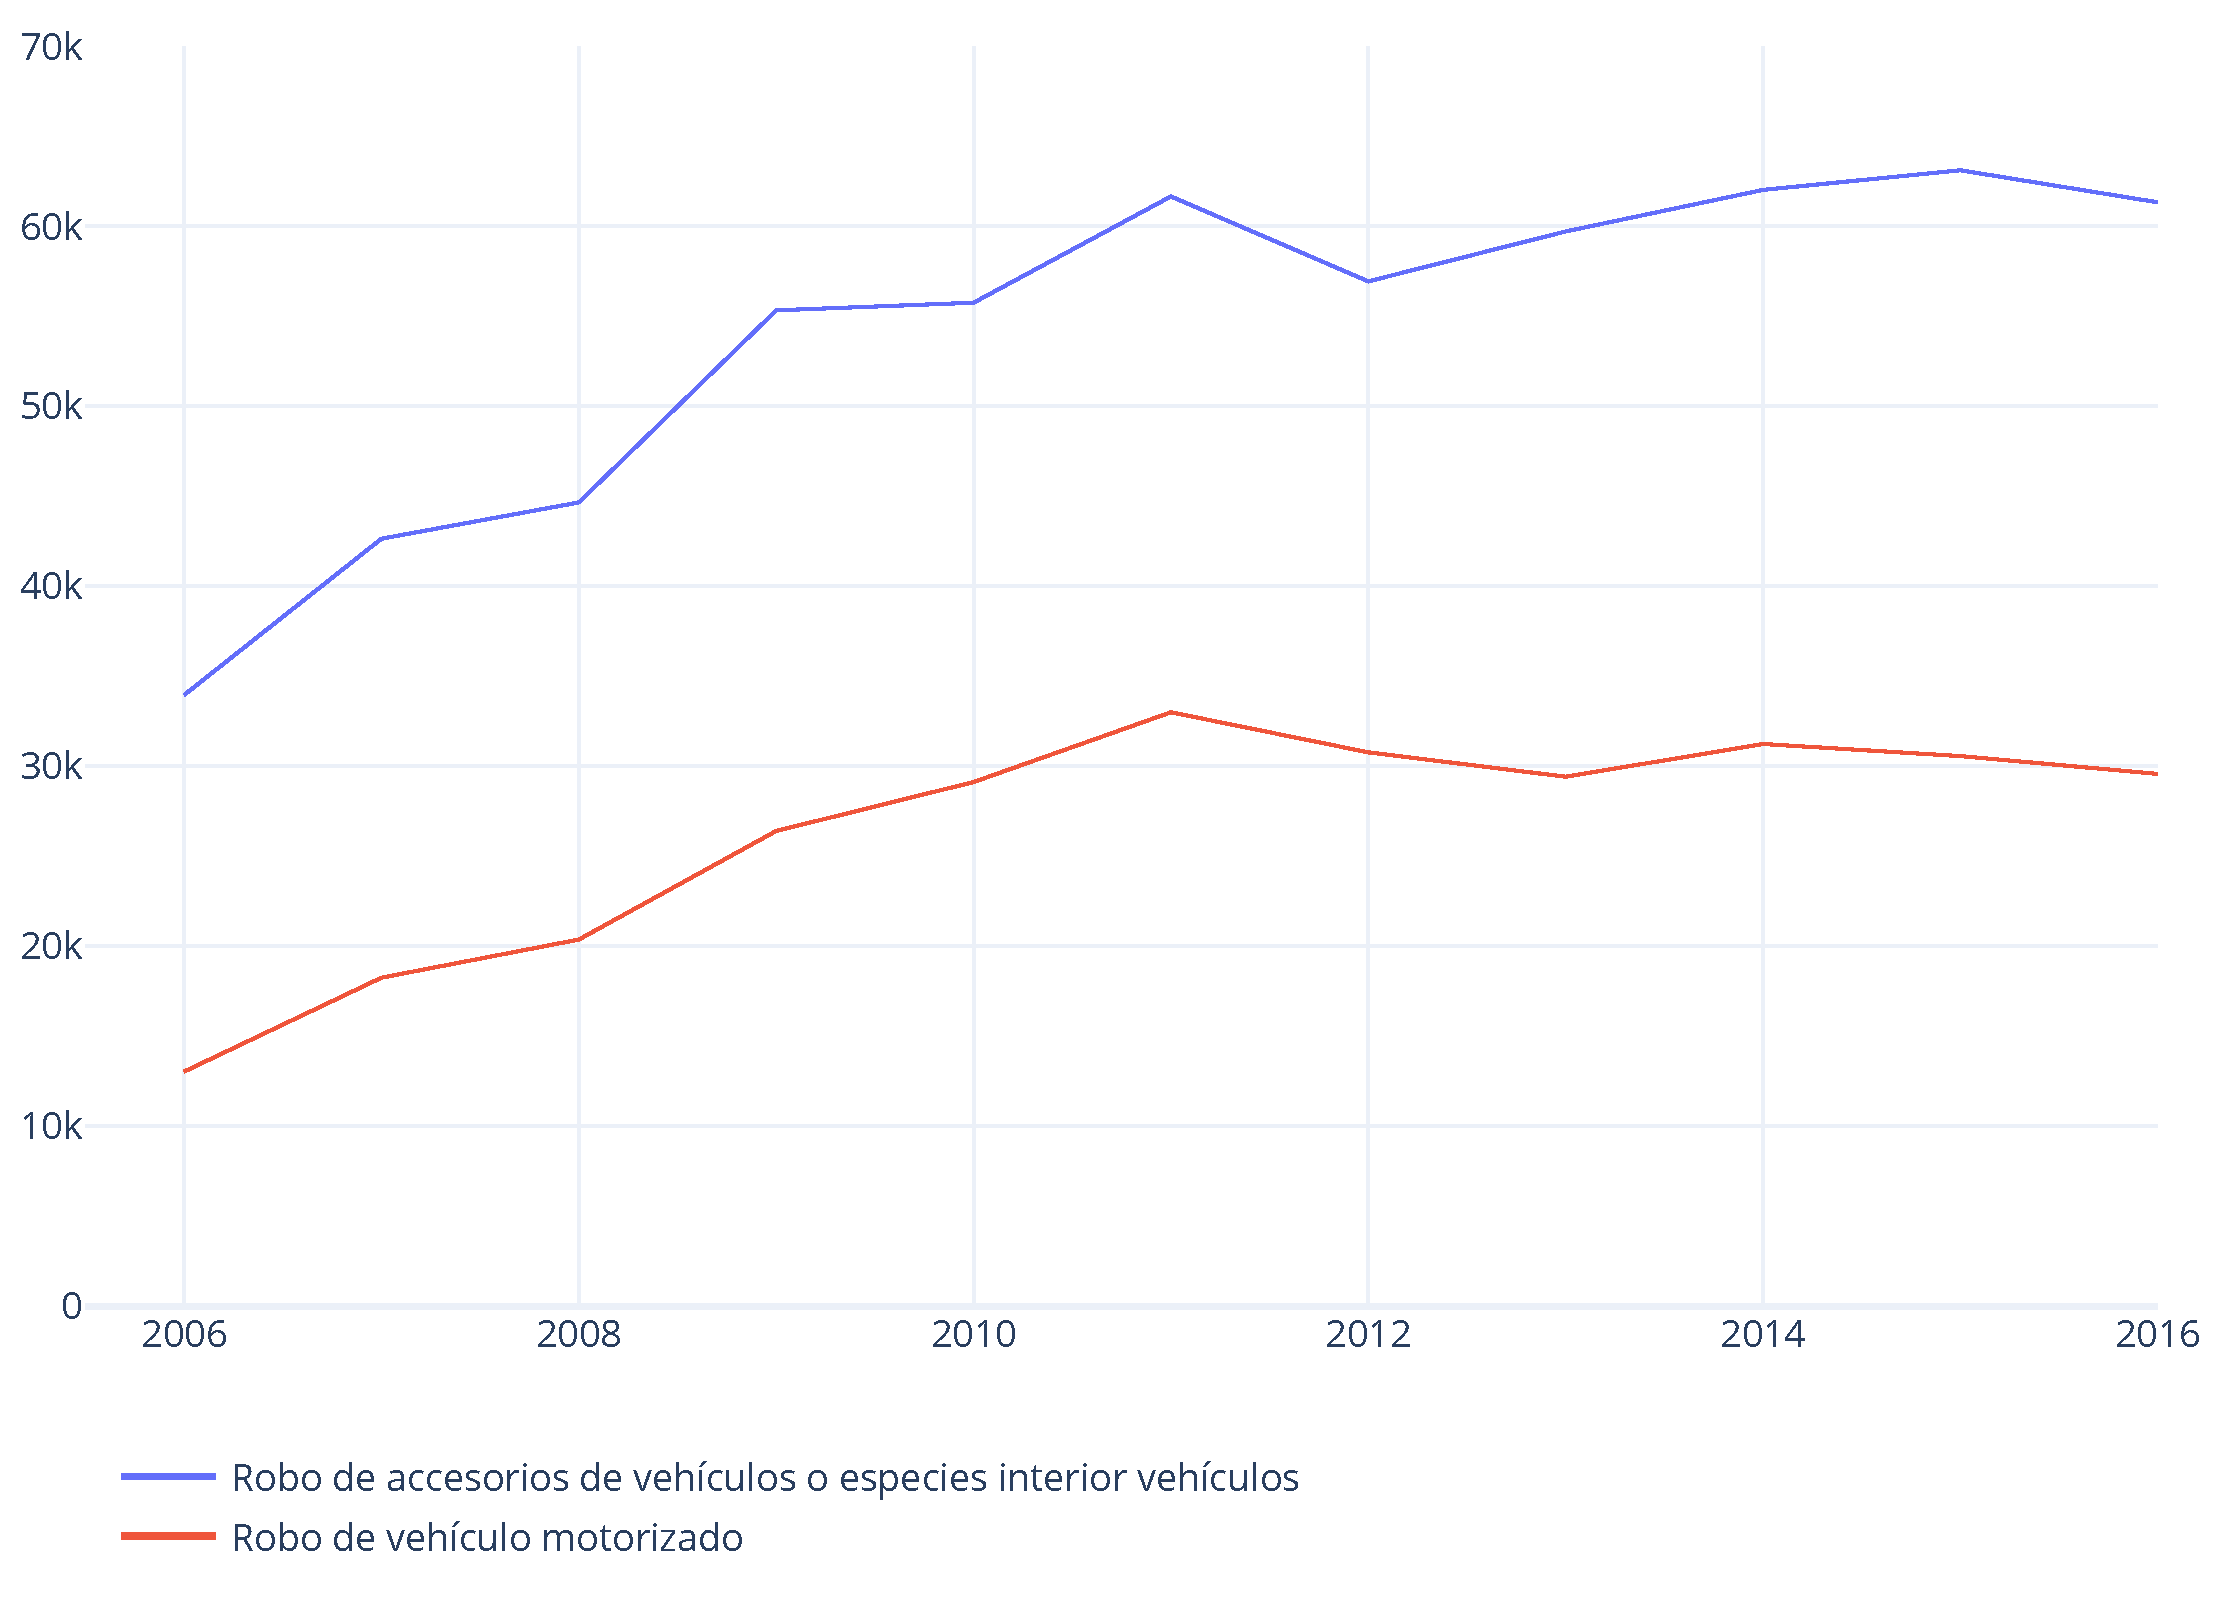
\includegraphics[width=1\textwidth]{ch1/robberies.eps} 
    \caption{Cantidad de robos de vehículos y accesorios anuales en Chile entre los años 2006-2016. Fuente: Informe anual Carabineros, 2006-2016, INE.} 
    \label{fig:antecedente}
\end{figure}

Este fenómeno trae consigo un montón de costos para la sociedad, como incremento en la percepción de la seguridad, aumentos en la prima de los seguros de los asegurados, aumento en los costos de las aseguradoras \footnote{Considerando que el costo promedio incurrido en un auto asegurado robado y no recuperado es de \$ 5.000.000 de pesos, la pérdida total considerando solo los vehículos no recuperados para el año 2015 es de unos \$15.720 millones de pesos.} y el incremento de otros tipos de delitos \footnote{El destino de los vehículos robados es variado, se usan los autos para perpetrar otros delitos y huir, venderlos por piezas en talleres clandestinos o blanquear sus documentos para pasarlos por la frontera y venderlos o cambiarlos por droga en el extranjero.}

El corpus utilizado correspode a una colección de 49015 relatos de víctimas de robo de vehículo, entre los años 2011-2016, provistos por la Asociación de Aseguradores de Chile (AACH). Cabe destacar que se estima que un tercio del parque automotriz se encuentra asegurado, por lo que se trabaja con una muestra del parque automotriz.\\
%http://www.economiaynegocios.cl/noticias/noticias.asp?id=185224

En el contexto de robo de vehículos, los tópicos vendrían siendo los \quotes{modu operandi} que utilizan los delicuentes para robar un vehículo. Así, la metodología propuesta permitiría descubrir los \textit{modus operandi} ocultos en los relatos de las víctimas y caracterizarlos a partir de las palabras, como también ver su evolución a través del tiempo, siendo capaz de detectar cuando nacen y mueren, y como cambian en el tiempo.\\

\section{Revisión del estado del arte}

El problema planteado consiste en un problema de \textit{clustering}, puesto que no se cuenta con una etiqueta del tema al que corresponde cada documento, siendo el propósito del trabajo descubrirla. Dentro de los métodos de \textit{clustering} que involucran texto el modelamiento de tópicos es uno de los enfoques más prometedores.\\

El modelamiento de tópicos es una poderosa herramienta que nos permite analizar grandes colecciones de documentos. En procesamiento de texto, un documento es una colección de palabras y el conjunto de documentos lleva por nombre corpus. Estos modelos encuentran los temas (\textit{clusters}) ocultos presentes en el corpus, permitiendo resumir, organizar y explorar grandes colecciones de datos.\\

Algunas de las técnicas de modelamiento de tópicos están basadas en factorización matricial como LSI (Latent Semantic Indexing) \citep{dumais2004latent} o NMF (Non-negative Matrix Factorization)\citep{xu2003document}, pero en este trabajo está basado en modelos probabilísticos generativos, como LDA (Latent Dirichlet Allocation)\citep{blei2003latent} o HDP (Hierarchical Dirichlet Process)\citep{teh2005sharing}. Ambos enfoques tienen sus pros y contras, en este trabajo se prefiere el enfoque probabilístico ya que es capaz de expresar incertidumbre en la asignación de un tópico a un documento y en la asignación de palabras a los tópicos, además, este enfoque suele aprender tópicos más descriptivos \citep{stevens2012exploring}.\\

En el modelamiento de tópicos se pueden presentar los siguientes dinamismos:
\begin{enumerate}
    \item \textbf{Evolución de los tópicos}: la evolución de los tópicos se refleja en el cambio en la distribución sobre las palabras. Por ejemplo, el \quotes{portonazo} en un determinado momento se comete en grupos de 2-3 personas con arma blanca, luego evoluciona de arma blanca a arma de fuego y lo perpetran jóvenes menores de edad.
    \item \textbf{Dinámismo en la mezcla de tópicos}: esto permite capturar la popularidad de los tópicos en el tiempo.
    \item \textbf{Nacimiento, muerte, fusión y división de tópicos}: En el contexto de robos es natural que en el tiempo aparezcan nuevos \textit{modus operandi} como también que desaparezcan aquellos que ya no parecen tan atractivos.
\end{enumerate}

En el modelamiento de tópicos estático destaca LDA y HDP. La diferencia principal en estos dos modelos es que el primero necesita de antemano fijar el número de tópicos a descubrir y el segundo lo infiere a partir del corpus.\\

Dentro de los primeros modelos de tópicos dinámicos que fueron exitosos podemos encontrar a Dynamic Topic Modelling (DTM) junto Topic Over Time (TOC)\citep{wang2006topics}. Estos modelos mantienen el número de tópicos fijo en el tiempo, por lo que si aparece un nuevo tópico este quedará clasificado dentro de un tópico preexistente desde el comienzo, por lo que solo es capaz de capturar el punto 1 y 2.\\

En \citep{ahmed2012timeline} se propone Dynamic Hierarchical Dirichlet Process (DHDP), modelo que no mantiene el número de tópicos fijo en el tiempo, sino que lo infiere a partir del corpus. Sin embargo, este modelo no es capaz de capturar fusión y división de tópicos. Además, a diferencia de los otros modelos de tópicos mencionados, DHDP no es una tecnología ampliamente usada y no cuenta con una implementación disponible, por lo que se desconoce su desempeño en otras fuentes de información.\\

En \citep{wilson2011tracking} y \citep{beykikhoshk2018discovering} se propone una metodología que permite capturar los dinámismos mencionados utilizando LDA y HDP respectivamente. Estas consisten en dividir el corpus en épocas, entrenar de forma independiente un modelo de tópico en cada época, para finalmente unir los resultados obtenidos. En este trabajo se utilizan técnicas de modelado dinámico de tópicos bajo este enfoque, usando como HDP para el descubirmiento de tópicos en cada época.

\section{Estructura de la tesis}
En el capítulo \ref{ch:theorethical_framework} se describen los fundamentos teóricos en los que se basa la metodología propuesta la cual es descrita en el capítulo \ref{ch:methodology}. Luego, en el capítulo \ref{ch:case_study} se presenta un análisis cuantitativo y cualitativo de la metodología propuesta al fenómeno de robo de vehículos. Finalmente, en el capítulo \ref{ch:conclusion} se presentan las conclusiones y futuras lineas de investigación.